\section{O Artefato AuditEdu-XAI}
\label{sec:artefato}

\subsection{Arquitetura Desacoplada}
\label{sec:arquitetura}

Treinar modelos com validação cruzada, calcular valores SHAP para milhares de instâncias e executar 240 retreinamentos são tarefas incompatíveis com uma interface que deve responder em menos de 2~s em servidores gratuitos de nuvem, tipicamente com poucos núcleos. A solução é uma \textbf{arquitetura desacoplada em duas camadas} (Figura~\ref{fig:arquitetura}): a \textbf{camada offline} executa todo o processamento pesado em lote e materializa os resultados como arquivos Parquet estáticos; a \textbf{camada online} apenas lê e apresenta esses arquivos, sem treinar modelos nem calcular valores SHAP em tempo de requisição. O contrato entre as camadas resume-se aos arquivos em \texttt{data/outputs/}, o que permite evoluir cada uma de forma independente.

\begin{figure}[htbp]
\centering
\begin{tikzpicture}[
    scale=0.9, transform shape,
    font=\footnotesize,
    node distance=4mm and 6mm,
    mod/.style={draw, rounded corners=2pt, fill=blue!6, minimum width=3.0cm, minimum height=9mm, align=center},
    store/.style={draw, cylinder, shape border rotate=90, aspect=0.18, fill=gray!10, minimum width=2.6cm, minimum height=10mm, align=center},
    ui/.style={draw, rounded corners=2pt, fill=green!8, minimum width=3.0cm, minimum height=9mm, align=center},
    arr/.style={-{Stealth[length=2mm]}, thick},
]
% Camada offline
\node[store] (raw) {Microdados\\ENEM (CSV)};
\node[mod, right=of raw] (etl) {\texttt{01\_etl}\\blocos + absenteísmo};
\node[mod, right=of etl] (pre) {\texttt{02\_preprocessing}\\moda, NMG, amostra};
\node[mod, below=of pre] (trn) {\texttt{03\_trainer}\\XGBoost + GridSearch};
\node[mod, left=of trn] (aud) {\texttt{04\_audit\_engine}\\teste: DI, TPR, SHAP};
\node[mod, left=of aud] (inj) {\texttt{05\_bias\_injection}\\validação (240 execuções)};
\node[store, below=8mm of aud] (out) {\texttt{data/outputs/}\\Parquet estático};
% Camada online
\node[ui, below=10mm of out] (app) {\texttt{app.py}\\Streamlit (cache)};
\node[ui, right=of app] (user) {Usuário\\(navegador)};
\node[draw, dashed, rounded corners, fit=(app)(user), inner sep=3mm, label={[font=\footnotesize\bfseries]below:Streamlit Community Cloud ou contêiner Docker}] (dock) {};
% Fluxos
\draw[arr] (raw) -- (etl);
\draw[arr] (etl) -- (pre);
\draw[arr] (pre) -- (trn);
\draw[arr] (trn) -- (aud);
\draw[arr] (aud) -- (out);
\draw[arr] (trn.south) |- ++(0,-4mm) -| (inj.south);
\draw[arr] (inj.south) |- (out.west);
\draw[arr] (out) -- node[right, font=\scriptsize]{leitura} (app);
\draw[arr, <->] (app) -- (user);
\begin{scope}[on background layer]
\node[draw=blue!40, fill=blue!2, rounded corners, fit=(raw)(etl)(pre)(trn)(aud)(inj)(out), inner sep=3mm, label={[font=\footnotesize\bfseries, anchor=south west]north west:Camada offline (lote)}] {};
\end{scope}
\end{tikzpicture}
\caption{Arquitetura desacoplada do AuditEdu-XAI}
\label{fig:arquitetura}
\fonte{Elaborado pelos autores.}
\end{figure}

A camada offline, implementada em Python~3.12 com pandas~2.3.3, PyArrow, scikit-learn~1.9.1, XGBoost~3.4.1 e SHAP~0.49.1, compõe-se de quatro módulos sequenciais (ingestão e filtro de absenteísmo; imputação, NMG e amostragem; treinamento; e motor de auditoria) e quatro complementares (injeção de viés, medição do tempo de resposta da interface, qualidade dos dados e manifesto de integridade). Cada módulo persiste sua saída em disco, o que permite reexecutar qualquer etapa isoladamente e inspecionar seus resultados. O módulo de injeção importa a função de cálculo de equidade do motor de auditoria, de modo que o indicador validado pelo experimento é exatamente o exibido pela ferramenta.

\subsection{Interface Interativa}
\label{sec:interface}

A camada online foi implementada com o Streamlit para um usuário sem formação em aprendizado de máquina, como um gestor, um professor ou um membro de órgão de controle, seguindo quatro princípios: \textbf{rótulos legíveis}, com os termos do dicionário do INEP (por exemplo, ``Sem computador em casa'' em vez de \texttt{Q024\_A}); \textbf{explicação em contexto}, com dicas e textos de interpretação; \textbf{acessibilidade}, com todo estado comunicado por ícone e texto, além da cor; e \textbf{honestidade estatística}, com intervalos de confiança e aviso de baixa precisão para grupos com menos de 30 casos positivos. Uma barra lateral seleciona a edição e o atributo protegido, e quatro cartões sintetizam a auditoria: o menor DI, o número de grupos em alerta, a taxa de seleção global (rotulada como ``acima da mediana da edição'', para evitar a leitura de ``aprovação'') e a AUC-ROC. A aba \textbf{Visão Geral de Equidade} (Figura~\ref{fig:dash_equidade}) mostra o DI de cada subgrupo com IC95\%, confronta o DI dos rótulos com o das previsões, traz TPR, FPR, download em CSV, uma nota que apresenta a regra dos quatro quintos como indicador de triagem e a evolução do DI entre 2019 e 2021. A aba \textbf{Explicabilidade (SHAP)} exibe a importância global e, para um candidato escolhido, o perfil socioeconômico, a chance estimada de ficar acima da mediana e um \textit{waterfall plot}. Esse recurso pode subsidiar, sem substituir, as informações sobre critérios e procedimentos a que o titular tem direito pelo Art.~20 da LGPD \cite{brasil2018lgpd}, pois uma decomposição técnica não equivale, por si só, a uma explicação clara e adequada ao destinatário leigo. A aba \textbf{Injeção Sintética de Viés} mostra a queda do DI nos cenários de injeção e de controle e a variação, muito menor, da AUC-ROC.

\begin{figure}[htbp]
\centering
% Recortes (trim = esquerda base direita topo, em px da captura 1440x2125):
% faixa de indicadores e gráfico de DI com IC95%.
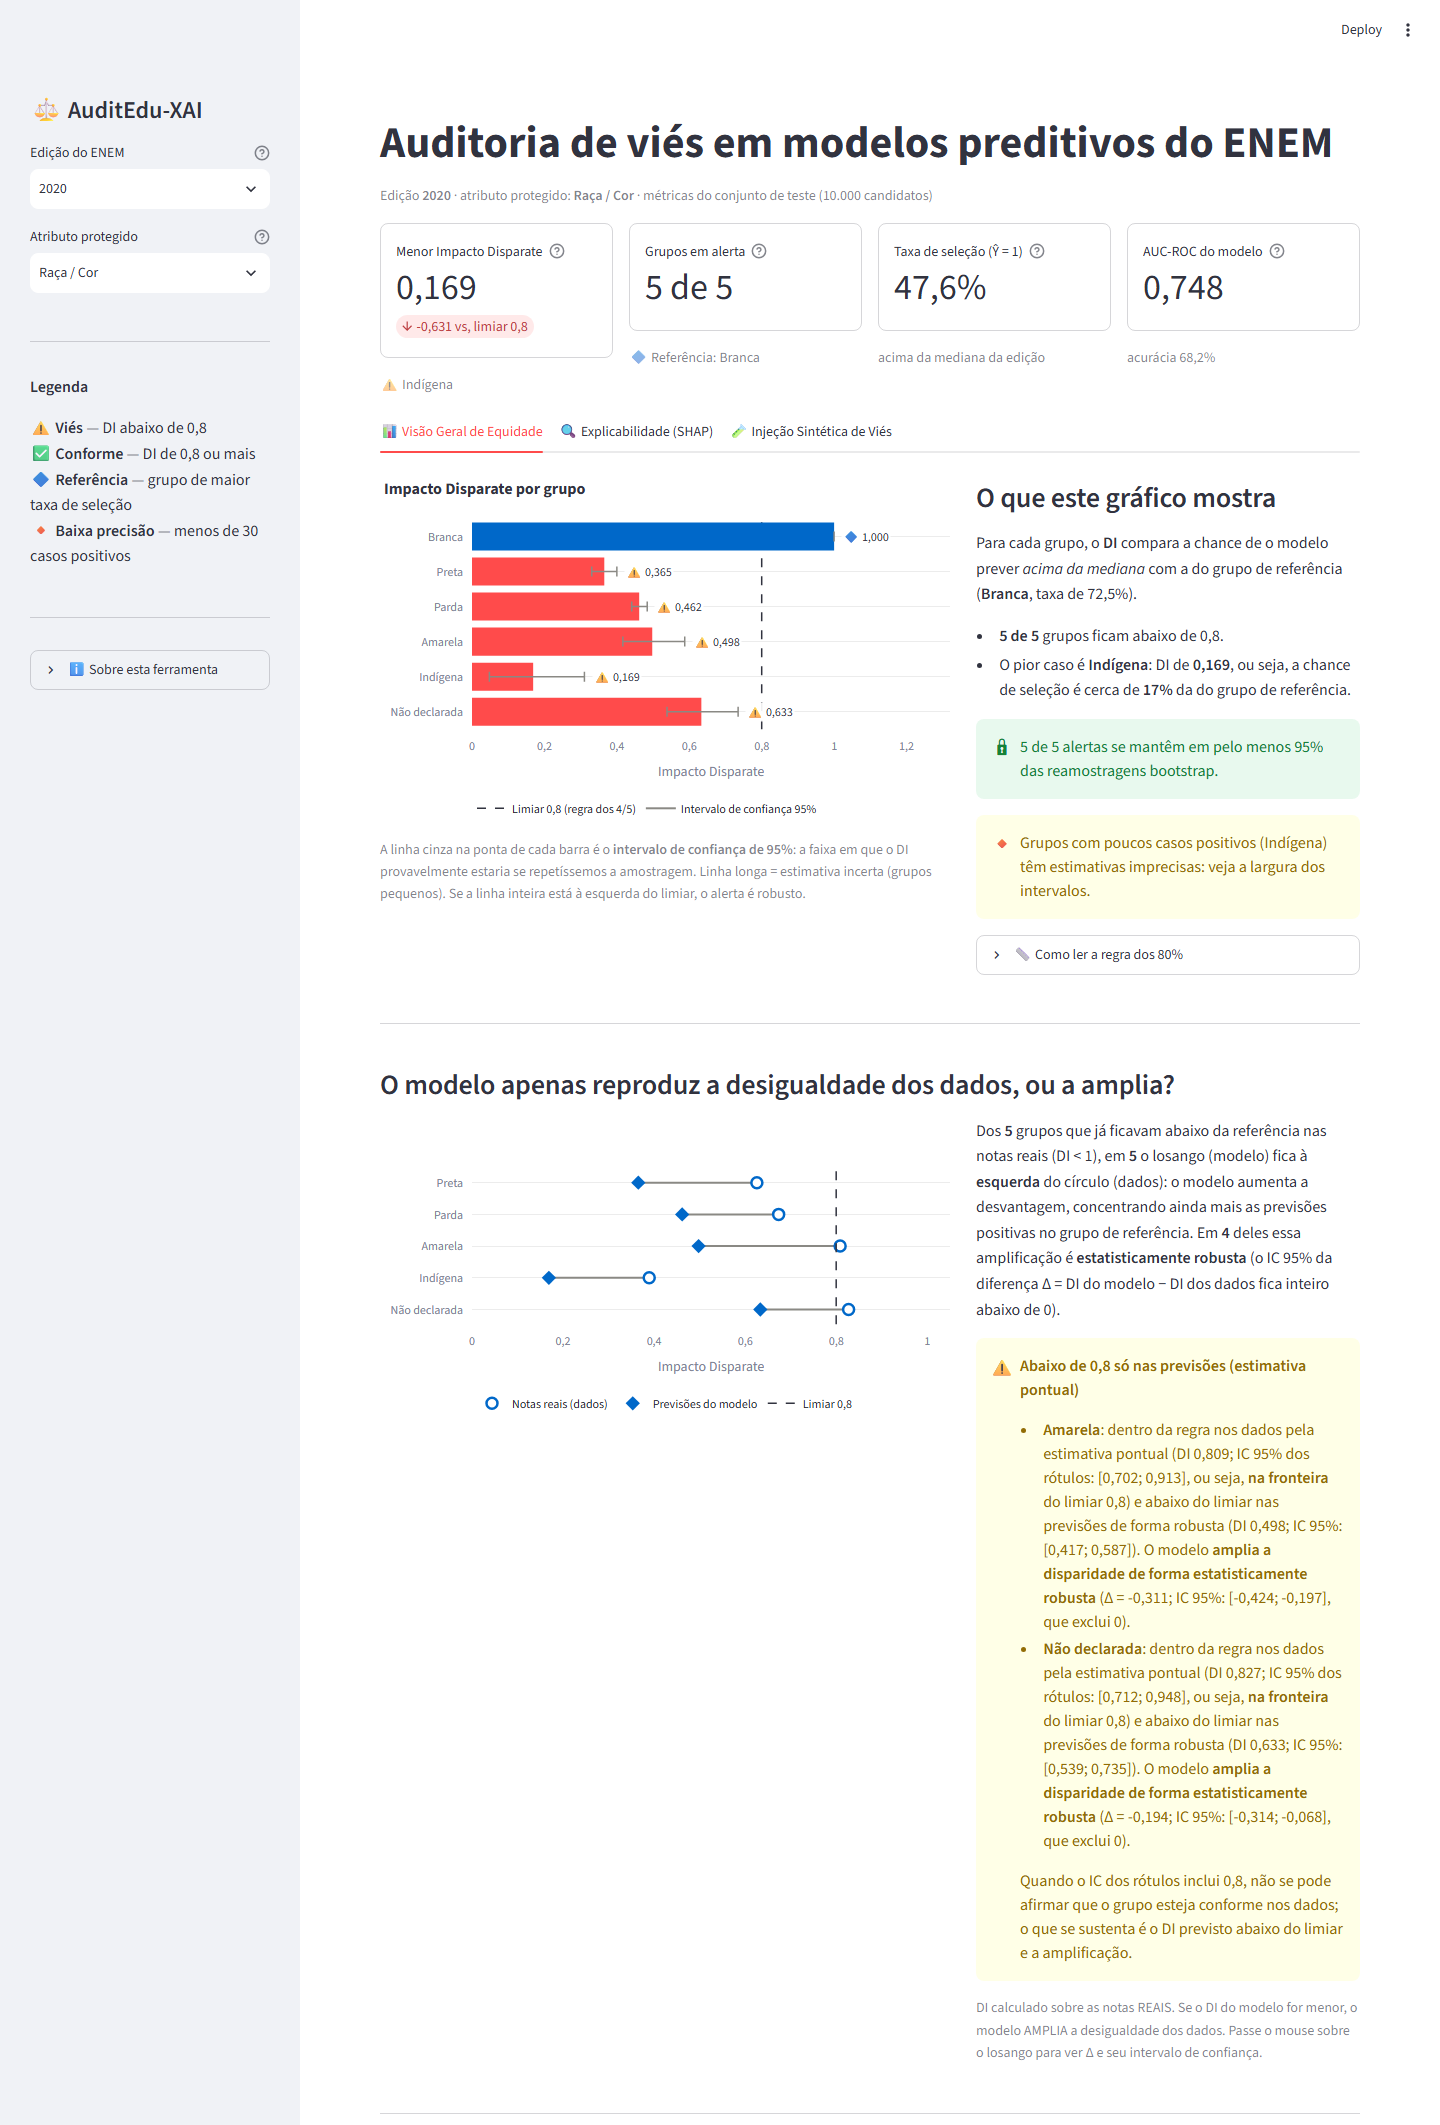
\includegraphics[width=\textwidth,trim=370 1727 70 215,clip]{../article/figuras/dashboard_equidade.png}\\[4pt]
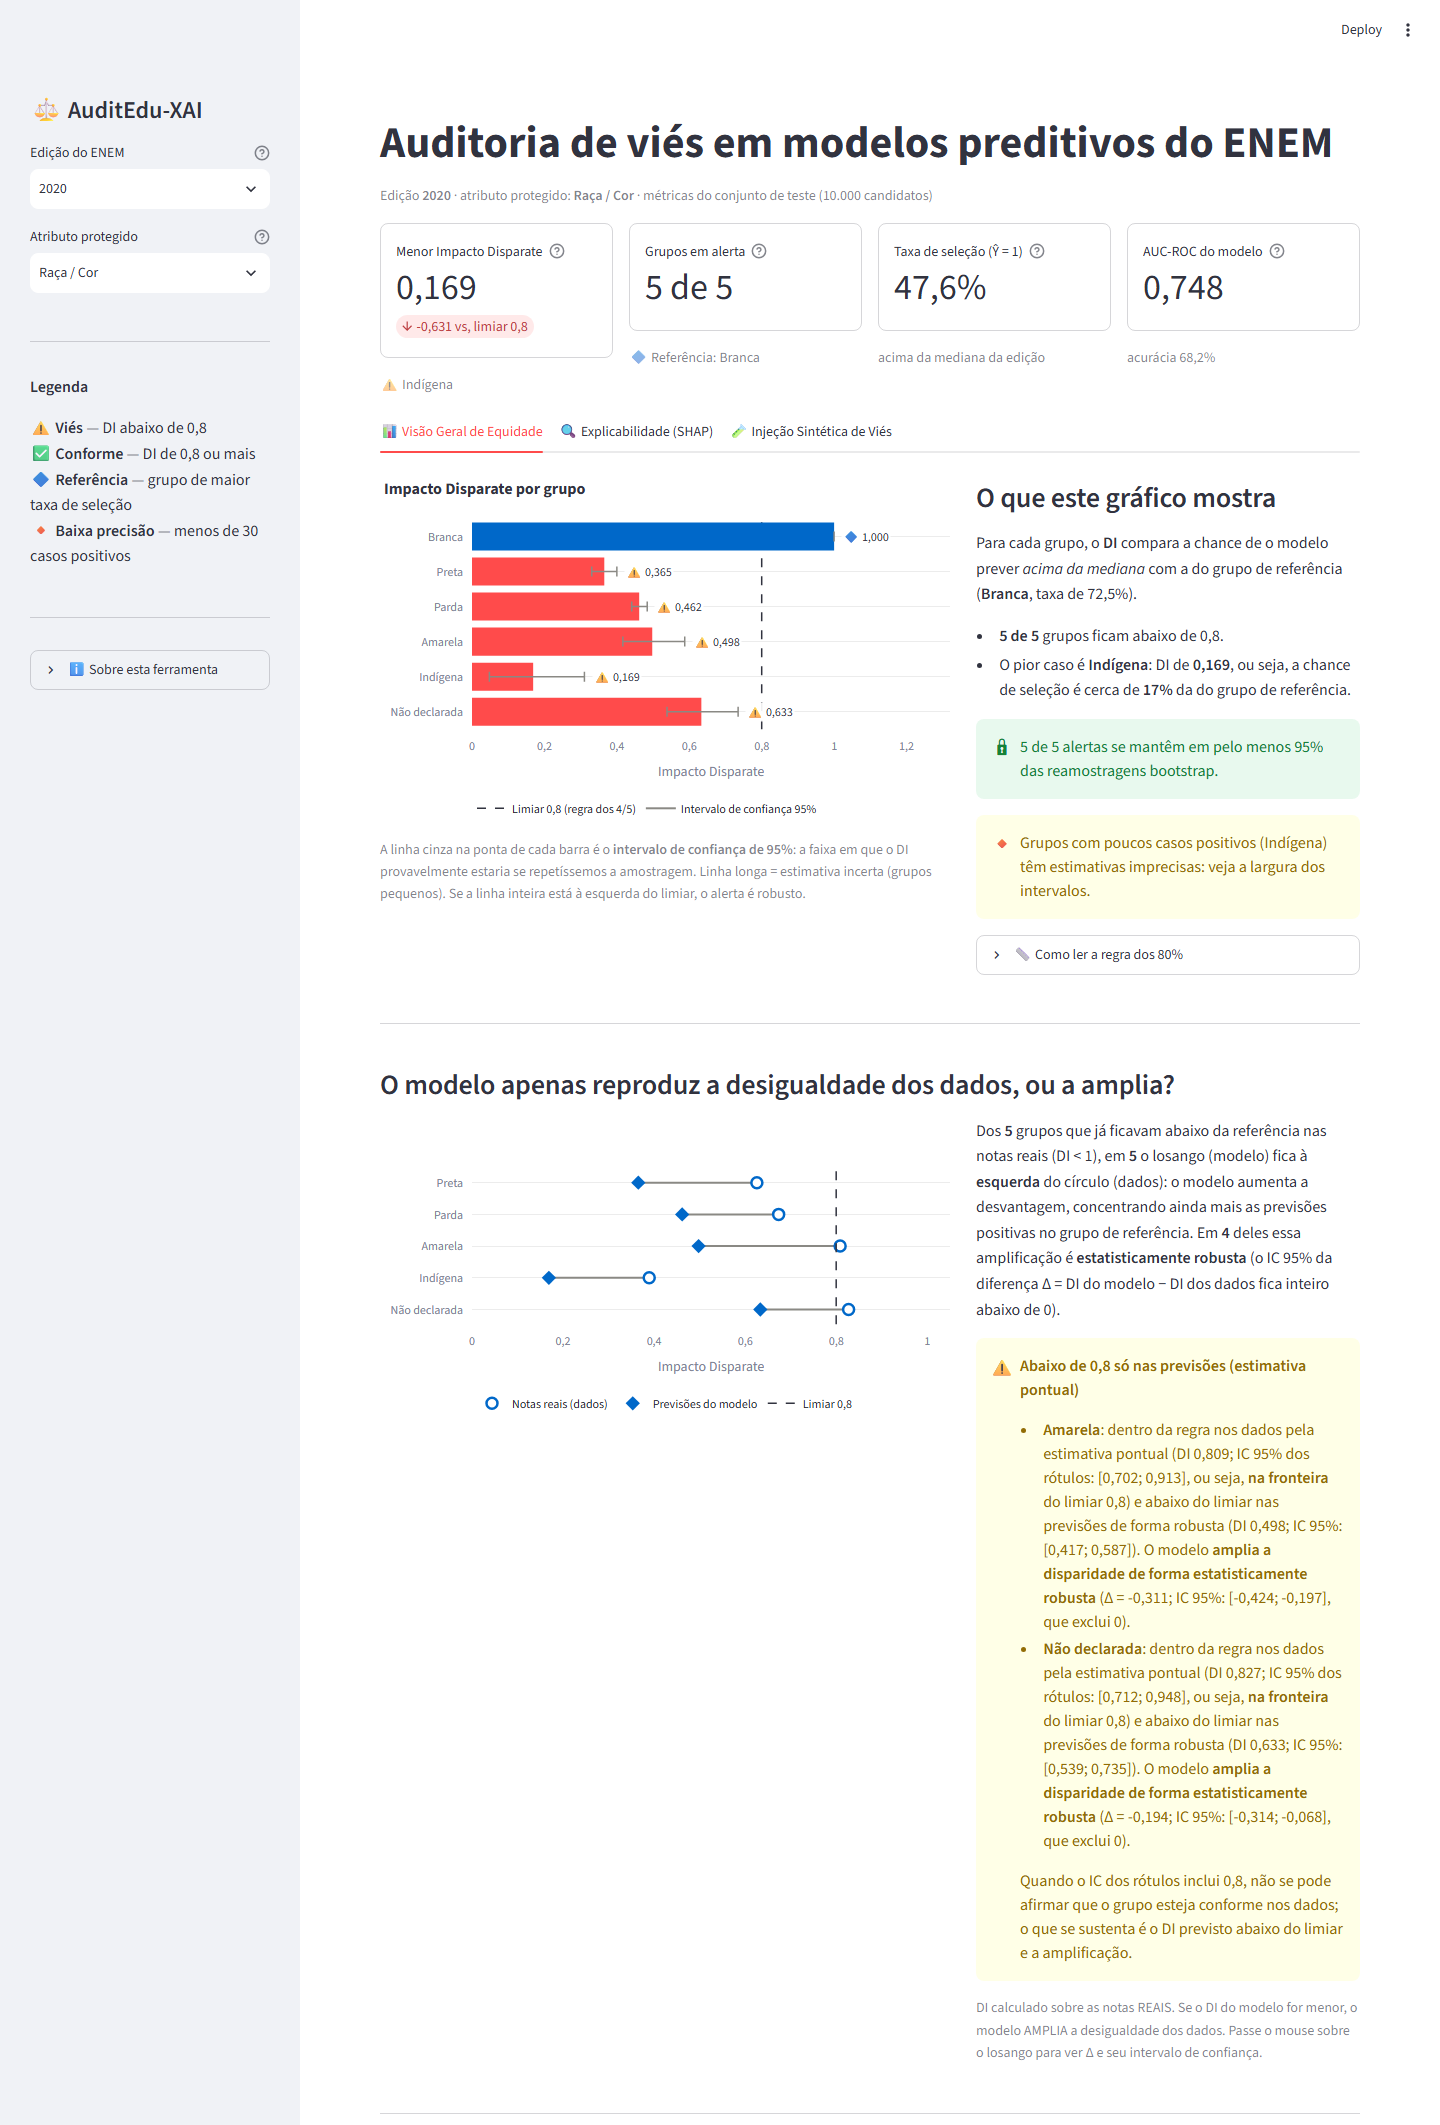
\includegraphics[width=0.8\textwidth,trim=375 1295 482 470,clip]{../article/figuras/dashboard_equidade.png}
\caption{Interface: indicadores e gráfico de DI da aba ``Visão Geral de Equidade'' (ENEM 2020, raça/cor; recortes da captura)}
\label{fig:dash_equidade}
\fonte{Elaborado pelos autores (captura da interface).}
\end{figure}

\subsection{Implantação, Desempenho e Reprodutibilidade}
\label{sec:implantacao}

A interface está implantada publicamente no Streamlit Community Cloud, serviço gratuito, em \url{https://auditeduxai.streamlit.app/}. A arquitetura desacoplada é o que viabiliza a hospedagem gratuita; como limitação operacional, aplicações sem acesso por 12 horas são hibernadas e demandam alguns segundos para reativação. A interface também é empacotada em uma imagem Docker de dois estágios, que contém apenas as dependências da interface, o código e os Parquets e executa como usuário não privilegiado. A imagem é validada por integração contínua (GitHub Actions) a cada alteração: o \textit{workflow} constrói a imagem, executa o contêiner limitado a 2 CPUs, aguarda o \textit{health check} e executa a interface completa em modo \textit{headless} para as três edições e os dois atributos, falhando se ocorrer qualquer exceção.

Os Parquets consumidos pela interface ocupam menos de 1~MB por edição, e dois níveis de cache evitam releituras e o redesenho do \textit{summary plot}, a operação mais cara da página, que por isso é exibido sob demanda. O tempo de resposta foi medido localmente executando a interface em modo \textit{headless} para cada edição e atributo (uma primeira carga e cinco interações), sem restrição e com a afinidade do processo restrita a 2 núcleos. Sem restrição, a primeira carga levou entre 0,17~s e 0,35~s; com 2 núcleos, entre 0,19~s e 0,33~s; nas duas configurações, as interações levaram em média entre 0,12~s e 0,19~s, com máximo de 0,280~s, e todas as 72 execuções ficaram abaixo de 2~s. A medição cobre a página na configuração padrão; a primeira renderização do \textit{summary plot}, acionada sob demanda, não está incluída. Essa medição é uma \textbf{aproximação} de um ambiente de nuvem com poucos núcleos, executada na mesma CPU física e sem a contenção de uma plataforma compartilhada; como a plataforma pública não divulga os recursos alocados, o tempo de resposta e o consumo de memória em produção não foram medidos.

Todas as etapas estocásticas usam a semente 42 ou geradores dela derivados, as versões das bibliotecas são fixadas, e um manifesto registra os \textit{hashes} SHA-256 dos dados, modelos e saídas. As tabelas e figuras de resultados deste artigo não são transcritas manualmente: um \textit{script} lê os Parquets e gera o código \LaTeX\ correspondente, de modo que qualquer divergência entre texto e artefato torna-se detectável.
